%!TEX root = ../BPlusTree-report.tex
\section{Background}
\label{sec:Background}
% Notes:
% What is a bplustree:
%   - Inherently imperative data structure
%   - Suboptimal implementation
%     - Running time of optimal implementation
%     - Running time of our implementation
%       - Mention how one could make it optimal.
%       - A tree in a tree in a tree, dawg
%     - Running time out of scope

\subsection{Gallina}
Gallina is a purely functional language\todo{ref}, which is used by the Coq interactive proof assistant. It is very lean, and does not include non-functional data structures, such as arrays\todo{ref}.

\subsection{B+ tree}
\label{subsec:Background_Bplus_tree}
The B+ tree is a n-ary, self-balancing, tree data structure\,\cite[pp. 334]{ramakrishnan2003database}, similar to a B-tree. It is composed of a root, nodes, and leaves. The root may be a leaf or a node. Nodes hold pairs of keys and pointers, $(k, p)$. $p$ points to either a node or leaf that holds the values over $k$, but below the key of the next pair. Leaves hold pairs of keys and values, $(k, v)$. In this project keys are always natural numbers, while values can have any type, denoted by $X$. In this project duplicate keys are not allowed.

\begin{figure}
 \centering
   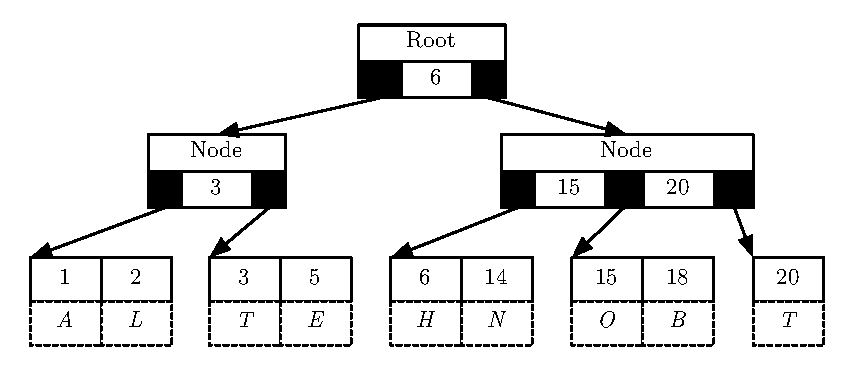
\includegraphics[width=90mm]{diagrams/BPlusTree.pdf}
 \caption{An example of a B+ tree with $b=1$. The bottom row contains leaves, with values, in this case characters, in the dashed boxes.}
 \label{fig:bplustree}
\end{figure}

For a given B+ tree, an order $b$ determines the capacity of nodes and leaves. A node must have at least $b+1$ children, and at most $2b+1$. A leaf must have between $b$ and $2b$ values. This rule is relaxed for the root node, which must have between 2 and $2b+1$ children. If the root is a leaf, it must have between 0 and $2b$ values\,\cite[p. 335]{ramakrishnan2003database}.

\paragraph{}
In our implementation, a node is a list of key-pointer $(k, p)$ pairs where $p$ points to a child tree. A leaf is a list of key-value $(k, v)$ pairs. We support three operations, which we will refer to as our primary operations. These are: insert, search and height. The theory behind the height function is trivial, and will not be explained in this section, but the theory behind the insertion and search functions require some explanation. Beyond these primary operations, we have also implemented a simple in-order traversal, for which it is worth noting that pointers between leafs for a speed-up in sequential access (range queries), which some implementations of B+ trees include, has not been implemented. The in-order traversal will not be mentioned further in this report. \todo{deletion?}

\subsubsection{Search}
\label{subsec:Search}
\todo{Mention running time of this operation}
The search function takes two arguments: a search key $sk$, and a tree $t$, to search in. Tree can be either a node or a leaf. If the the tree is a node, the function finds the pointer $p$ in the node for which it holds that
\begin{itemize}
	\item $p$ is the start pointer of the node and there exists a key $k$ that immediately succeeds $p$, where $sk < k$ OR
	\item There exists keys $k1$ and $k2$ on each side of $p$ and $k1 <= sk < k2$ OR
	\item $p$ is the end pointer of the node and for all keys $k$ in the node $k <= sk$
\end{itemize}
The function then recursively calls itself with the subtree $p$. Once the function reaches a leaf, the function searches for the key-value pair. This is often implemented as binary search in an array. 

\subsubsection{Insert}
\todo{Mention running time of this operation}
The insert function takes two arguments: a key-value pair $(k, v)$ and a tree $t$ to insert the pair into. The function starts at the root of the tree, and recursively searches for the leaf to insert into. It does this search in the same way the Search operation does it. The pair is then inserted into the leaf at the correct position. If the insertion results in the leaf having more than $2b$ values, the leaf must be split. This is called a leaf overflow. This is handled by splitting the leaf in half, and inserting a pointer to the new leaf in the parent node. If the parent node now has more than $2b$ children, it most also be split, following the same pattern. This can continue all the way to the root, which in turn can be split into two. If this happens, a new root node is created, as a parent to two split halves of the old root, and the height of the tree increases by one. Thus, a B+ tree can be seen to grow up from the leaves and is always in perfect balance.
